\documentclass[12pt, a4paper]{article}
\usepackage{geometry}
\usepackage{booktabs}
\usepackage{diagbox}
\usepackage{graphicx}
\usepackage{tabularx}
\parindent 0pt
\parskip 5pt
\pagestyle{plain}

\title{\textsc{Consensus}}
\author{}
\date{}

\begin{document}
\maketitle


\section{Motivation}

Achieving agreement among remote processes (where some may be faulty) is a
fundamental problem in distributed computing \cite{fischer1985impossibility}.
This problem is known as \textit{consensus} and lies ``at the core of many
algorithms for distributed data processing, distributed file management, and
fault tolerant distributed applications.'' \cite{fischer1985impossibility}

Due to issues such as node failures and network unreliability, it is difficult
to achieve consistency among nodes in distributed computing or multi-agent
systems.

\section{Formal Definition}

\subsection{Consensus Problem}

The consensus problem is defined with respect to a collection of $N$ processes
which communicate by message passing. Every process $p_{i}$ $(i = 1, \ldots, N)$
begins in the \textit{undecided} state, in which they each propose a single
value $v_{i} \in D$, where $D$ is a set of acceptable values
\cite{coulouris2005distributed}.

The processes then exchange values with each other. During this phase, each
process sets the value of its \textit{decision variable}, $d_i$ $(i = 1, \ldots,
N)$, based on the information obtained from other processes. In doing so, they
enter the \textit{decided} state, in which the decision variable may no longer
change.

A consensus algorithm must satisfy the following conditions for every execution:

\begin{itemize}
  \item \textbf{Termination}: Each non-faulty process $p_i$ must eventually set
    $d_i$.
  \item \textbf{Agreement}: All non-faulty processes in the decided state
    must have the same value. If $p_{i}$ and $p_{j}$ are correct and have
    entered the decided state, then $d_{i} = d_{j}$ $(i, j = 1, \ldots, N)$.
  \item \textbf{Integrity/Validity}: If all non-faulty processes proposed
    the same value, then the decision variable of all non-faulty processes is
    that same value.
\end{itemize}

There are two other problems similar to the consensus problem---the
\textit{Byzantine generals problem} (also known as the \textit{Byzantine
agreement problem}) and the \textit{interactive consistency problem}. Table
\ref{tab:dbtap} provides a comparison between these and the consensus problem.
Despite the differences in requirements, a solution to any one of them can be
transformed to one of the others by reduction \cite{fischer1983consensus}.

\begin{table}[htp]
  \centering
  \begin{tabularx}{\linewidth}{lXXX}
  \toprule
  Condition & Consensus Problem & Byzantine Generals Problem
    & Interactive Consistency Problem \\
  \midrule
  \textbf{Termination} & Eventually decide on a \textit{value}
    & Eventually decide on a \textit{value}
    & Eventually decide on an \textit{array $A$} \\
  \addlinespace
  \textbf{Agreement} & Agree on the same value
    & Agree on the same value
    & Agree on the same array of values $A[v_{1} \ldots v_{n}]$ \\
  \addlinespace
  \textbf{Integrity}
    & The decision value is based on all the correct processes's propositions
    & If the commander is correct, then all correct processes decide
      on the value that commander proposed
    & All correct processes decide on $v_{i}$ as the ${i}$th component of their
      vector, if $p_{i}$ is correct \\
  \bottomrule
\end{tabularx}
  \caption{Comparison of similar problems}
  \label{tab:dbtap}
\end{table}

\subsection{CAP Theorem}

The CAP theorem \cite{brewer2012cap} states that, in a distributed system, it is
impossible for an algorithm to provide more than two of these three properties:

\begin{itemize}
	\item \textbf{Consistency}: All data backups in the distributed system have
    the same value at the same time.
	\item \textbf{Availability}: After some nodes in the cluster fail, the entire
    cluster can still respond to client read and write requests, but there is no
    guarantee that the data responded is most latest.
	\item \textbf{Partition tolerance}: The system continue to operate despite
    delayed, lost or dropped messages on the network.
\end{itemize}

%% Maybe include in the future.
% \subsection{ACID Theorem}

\subsection{Models of Computation}

The difficulty of solving consensus problem under different system models and
assumptions are varied. Each consensus algorithm has its assumptions about the
problem, and we need to classify and compare based on their assumptions about
the problem.

\subsubsection{Synchronous and Asynchronous Systems}

There are two most popular system models in distributed systems - synchronous
system model and the asynchronous system model. In the synchronous system model,
there is a bound on how long a message takes to be delivered, which means each
message is received within bounded time as long as the sender and recipient
processes are alive. The drift of each process's local clock has a known bound.
Each step in a process takes a time that is lower bounded by a known value and
upper bound by a known value. The bound is a global bound across the entire
state system. E.g., a collection of processors connected by a communication bus.
The asynchronous system model, on the other hand, does not have any bound on
anything. There is no bound on process execution and message transmission
delays. The drift rate of a clock might be arbitrarily fast or arbitrarily slow.
The asynchronous system is a more general model than the synchronous system
model, which also means the consensus problem is more difficult to be solved in
this model. An algorithm work for an asynchronous system will also work for the
asynchronous system. Lots of the very widely used distributed systems adhere to
it. In the synchronous system model, the consensus problem is solvable. However,
the consensus is impossible to solve in the asynchronous system model
\cite{fischer1985impossibility}. Whatever protocol or algorithm is provided,
there is always a worst-case possible execution scenario where some processes
fail, and some messages are delayed, which would prevent the system from
reaching consensus. But actually, this impossibility result derives from a
worst-case scenario that hardly happens. In reality, process scheduling has a
degree of randomness \cite{aguilera2010stumbling}. So, even though it is
theoretically feasible to provide consensus in the asynchronous system model,
through some compromises, practical asynchronous system consensus algorithms can
still be implemented in practice.

\subsubsection{Byzantine and Crash Failures}

According to the types of failures that consensus algorithms can handle, we can
classify them into the following two types:

\begin{itemize}
	\item Byzantine Fault Tolerance (BFT): A BFT Algorithm can handle fault in
    arbitrary ways, including malicious actions of an adversary.
	\item Crash Fault Tolerance (CFT): A CFT Algorithm can handle failure caused
    by processes crash or fail-stop. E.g., Paxos and Raft.
\end{itemize}

Any algorithm that can work for BFT would also work for CFT. That is because
Byzantine failures contain all possible faults in the system model. The relation
of different faults \cite{barborak1993consensus} is shown on Figure
\ref{fig:aofc}.

\begin{figure}[htp]
  \centering
  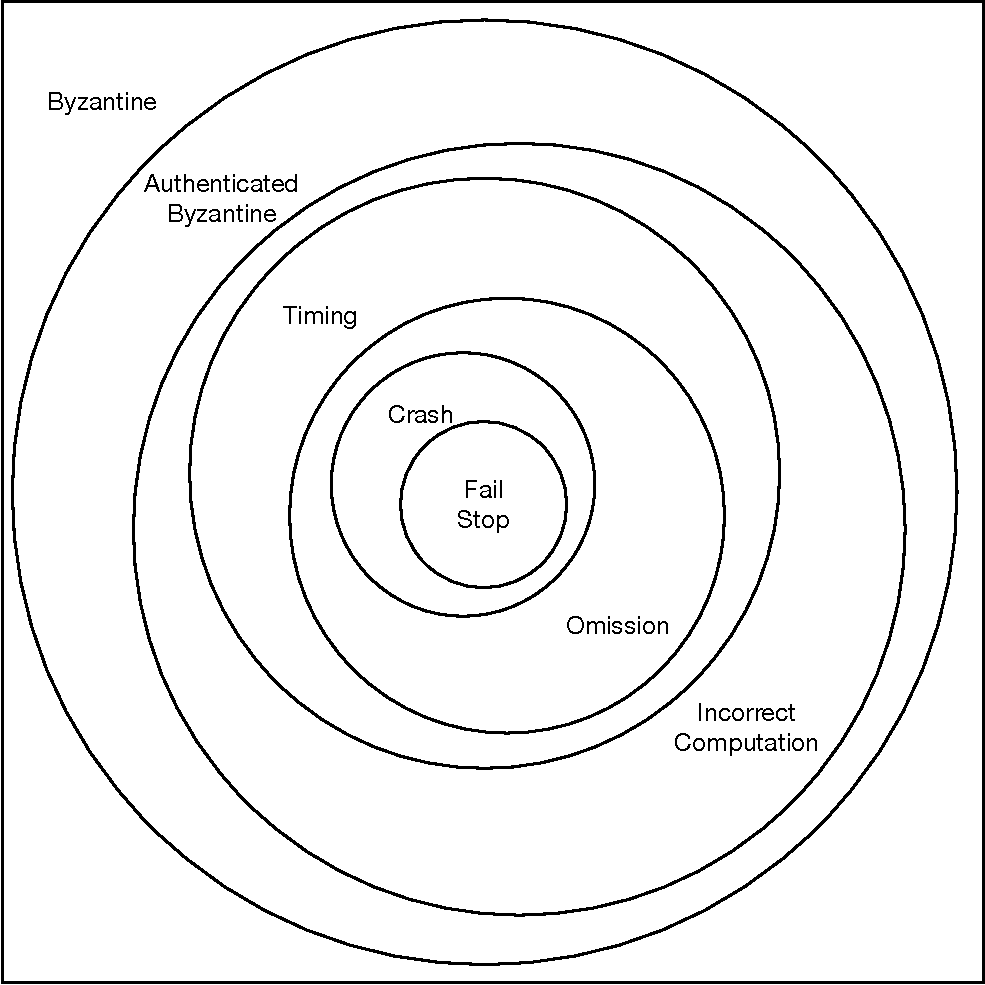
\includegraphics[width=0.8\textwidth]{img/AOFC.pdf}
  \caption{An ordered fault classification (\textbf{include author here})}
  \label{fig:aofc}
\end{figure}

\subsection{Consensus Algorithms}

Many problems in distributed systems are closely bound up with consensus, which
makes finding effective solutions to consensus problem become significant.

%% Aaron Yau: Maybe I would write this part next week, to give a brief summary
% and comparison of some well-known algorithms instead of paxos or rafe. Or I
% would feel appreciate that someone can continue to write based on the things I
% wrote.}


%% May be needed in the future.
% \section{Impossibility of consensus}
% It has been shown that in an asynchronous system of processes, ``every protocol
% for this problem has the possibility of nontermination, even with only one
% faulty process.'' \cite{fischer1985impossibility}


\section{Relevant problems}


\subsection{Reliable Multicast}

Ensuring that all processes receive updates in the same order.

\subsection{Membership/Failure Detection}

Ensuring that every process has a local record containing every other process.
Failures should be detected and records should be updated.

\subsection{Leader Election}

Deciding on a leader among all processes, with all processes being aware of
who the leader is.

\subsection{Mutual Exclusion}

Ensuring that simultaneous access to a resource does not occur (exclusive
access).


\section{Paxos algorithm}

\subsection{Roles}

A process can take more than one role.

A process is \textit{persistent}---it cannot forget what it has accepted.

  \subsubsection{Proposer}

  \subsubsection{Acceptor}

  \subsubsection{Learner}

\subsection{Protocol}

\subsection{Issues}

  \subsubsection{Contention}

\subsection{Optimisations}


\section{Raft algorithm}

\subsection{Roles}

\subsection{Issues}

\subsection{Optimisations}


\section{Comparative analysis}


\section{Application}


\bibliographystyle{ieeetr}
\bibliography{main}

\end{document}
